\newpage
\thispagestyle{empty}
\section{Einleitung Neuronale Netze}\label{sec:einleitung_nn}   

\vspace{1cm}

\begin{tcolorbox}[title={Inhalt}]
  \begin{quotation}\noindent
      Dieses Kapitel liefert einen Einstieg in neuronale Netze. Es werden an Beispielen unterschiedliche Anwendungsfälle anschaulich gemacht.
      Ebenso soll bereits eine grobe Idee näher gebracht werden, wie ein neuronales Netz aufgebaut ist.
      Insgesamt werden in diesem Kapitel bereits zahlreiche grundlegende Begriffe erklärt, die in den nachfolgenden Kapiteln benötigt werden.
  \end{quotation}
  \begin{itemize}  
    \item Wofür benötigt man Neuronale Netze?
    \item Einsatzgebiete
    \item Grobes Prinzip
  \end{itemize}
\end{tcolorbox}

\subsection{Wofür benötigt man Neuronale Netze?}\label{subsec:einleitung_nn:wofuer_nn}
Mit neuronalen Netzen lassen sich Probleme lösen, die mit herkömmlichen Algorithmen nur schwer bis gar nicht lösbar sind. Neuronale Netze sind grundsätzlich in der Lage, nicht lineare Abbildungen anzunähern, Beispiele folgen weiter unten (siehe \ref*{subsec:einleitung_nn:einsatzgebiete}).
Der große Vorteil neuronaler Netze liegt darin, dass sie selbstständig lernen können, komplexe Muster in großen Datenmengen zu erkennen, wodurch man die entsprechenden Algorithmen nicht mehr von Hand schreiben muss.

\bigbreak\noindent
Aufgrund ihrer Fähigkeit, schnell und effizient komplexe Muster zu erkennen, können neuronale Netze auch Aufgaben lösen, für die man normalerweise Menschen benötigen würde, da herkömmliche Algorithmen diese Probleme nicht zuverlässig genug lösen können oder der Entwicklungsaufwand unverhältnismäßig groß in Relation zum Nutzen wäre.

\bigbreak\noindent
Häufig sind Muster zu komplex, um sie mit einem klassischen Algorithmus erfassen zu können oder sie sind schlecht von Hand mathematisch formulierbar, wie zum Beispiel die Bilderkennung.
Mit Hilfe eines neuronalen Netzes kann man aber dennoch mit relativ geringem Aufwand ein Netz trainieren, das in der Lage ist, solche Bilderkennungsaufgaben zu erledigen.

\bigbreak\noindent
Neuronale Netze sind häufig auch zuverlässiger als klassische Algorithmen, da diese manchmal bestimmte Sonderfälle nicht abdecken, wohingegen neuronale Netze resistenter gegen fehlerhafte Daten und Rauschen sind und besser mit Sonderfällen umgehen können.

\subsection{Einsatzgebiete}\label{subsec:einleitung_nn:einsatzgebiete}
Neuronale Netze sind äußerst vielfältig und lassen sich für verschiedenste Anwendungen anpassen und trainieren.
Zu den häufigsten Anwendungsfällen zählen die Bilderkennung und die Verarbeitung von auditiven Daten.

\bigbreak\noindent
Die Bilderkennung mittels neuronaler Netze lässt sich beispielsweise dazu einsetzen, medizinische Diagnosen durchzuführen, da diese Netze fähig sind, komplexe Krankheitsbilder zu erkennen.
Auch kann die Bilderkennung genutzt werden, um die Position von Personen oder anderen Objekten auf einem Kamerabild zu identifizieren, was zur Realisierung von autonomem Fahren nützlich ist.
Die Bilderkennung mittels neuronaler Netze findet auch in der Industrie Anwendung, um hergestellte Produkte automatisiert auf Mängel zu prüfen und auszusortieren.

\bigbreak\noindent
Neuronale Netze können auch in Analytics Software eingesetzt werden, um das Nutzerverhalten auf einer Website zu analysieren und den Nutzern so zum Beispiel personalisierte Werbung oder bessere Videovorschläge bieten zu können.

\bigbreak\noindent
Grundsätzlich sind neuronale Netze in der Lage, beliebige Arten von Eingabedaten zu verarbeiten.
So ist es auch möglich, Audio-Daten zu verarbeiten und so beispielsweise Spracherkennung, automatisch generierte Untertitel und Sprachassistenten zu implementieren.

\subsection{Grobes Prinzip}\label{subsec:einleitung_nn_grobes:prinzip}
Neuronale Netze sind von der Funktionsweise menschlicher Gehirne inspiriert und versuchen dadurch eine ähnliche Lernfähigkeit zu erzielen.
Dabei werden Netze aus Neuronen simuliert, um menschliche Lernprozesse und kognitive Fähigkeiten nachzuahmen. 

\bigbreak\noindent
Die Neuronen neuronaler Netze sind in Schichten organisiert, die untereinander verbunden sind, wobei die Signale von Schicht zu Schicht durch das Netz geleitet werden.
Jedes einzelne Neuron eines Netzes verarbeitet seine Eingabedaten durch die Anwendung mathematischer Funktionen und leitet das Ergebnis dann an das nächste Neuron weiter.
Die Verbindungen zwischen den Neuronen sind von variabler Stärke und sind der primäre Faktor, der beim Lernprozess verändert wird.

\bigbreak\noindent
Neuronale Netze werden trainiert, indem man sie auf einen Trainingsdatensatz anwendet und die Verknüpfungen der Neuronen basierend auf der Stärke der Abweichung vom gewünschten Ergebnis anpasst.
Der Trainingsdatensatz enthält dabei beispielhafte Eingabedaten und die dazugehörige gewünschte Ausgabe.

\bigbreak\noindent
Nach dem Trainingsvorgang kann man das Netz dann auf ihm unbekannte Daten anwenden, wobei es dann eine Ausgabe basierend auf den erlernten Mustern bildet.


%Neuronen 
\newpage  
\section{Neuronen}\label{sec:neuronen}
  \begin{tcolorbox}[title={Inhalt}]
    \begin{quotation}\noindent
        Im letzten Kapitel wurde bereits ein Einblick in den Aufbau eines neuronalen Netzes gegeben. 
        Dieses Kapitel widmet sich Neuronen, deren Bedeutung in einem Netz und wie diese untereinander verknüpft sind.
        Es wird hier bereits die einfachste Form eines Neuralen Netzwerk vorgestellt.
    \end{quotation}
\begin{itemize} 
    \item Was sind Neuronen
    \item Arten von Neuronen
    \item Funktionsweise
    \item Aktivierungsfunktion
    \item Schichtenmodell
\end{itemize} 
\end{tcolorbox}
\subsection{Was sind Neuronen?}\label{sec:neuronen:was_sind_neuronen}  
Das menschliche Nervensystem besteht aus Neuronen, welche mit Axonen oder Dendriten verknüpft sind. Diese Verbindungen werden auch Synapsen genannt. Die variable Stärke der Synapsen
ermöglichen das Lernen. Dieser biologische Mechanismus wird durch neurale Netze simuliert.\\

\begin{figure}[H]
\begin{subfigure}{0.6\textwidth}
    \includegraphics[width=\textwidth]{Sources/01-01_synapse.png}
    \label{Synapse}
    \caption{Synapse}
\end{subfigure}
\begin{subfigure}{0.25\textwidth}
    \includegraphics[width=\textwidth]{Sources/01-02_neuron.png}
    \label{Neuron}
    \caption{Neurales Netzwerk}
\end{subfigure}
\caption{Bild aus dem Buch 'Neural Networks and Deep Learning' von Charu C. Aggarwal
}
\end{figure}
\noindent
Ein neuronales Netz besteht aus mindestens einem Neuron. Neuronen sind essentielle Bestandteile von neuralen Netzen. Sie nehmen Eingabedaten entgegen und wandeln diese 
in Ausgabedaten um. Neben den Eingabedaten werden auch Weight-Parameter übergeben, welche die zu berechnenden Werte beeinflussen. Das eigentliche \enquote{Lernen} erfolgt durch diesen 
Einfluss.\cite{CA18}
\subsection{Arten von Neuronen}\label{subsec:neuronen:arten_von_neuronen}
\subsubsection{Input Neuronen}
Input Neuronen erhalten Rohdaten und übergeben diese zusammen mit Weights an die Output Neuronen oder die versteckten Neuronen. Jedes Input Neuron ist mit jedem Neuron aus der nächsten Schicht 
(Hidden oder Output) verknüpft. Eine Aktivierungsfunktions entscheidet, ob das Neuron in der nächsten Schicht aktiviert werden soll. \cite{CA18}
\paragraph{Bias Neuronen}
Das Bias Neuron hat typischerweise den Wert 1. Das Produkt des Bias Neurons und dessen Weight wird auf die Summe der Neuronen aus der Input/Hidden Layer mit auf addiert. Das heißt, dass dieses Neuron
das Ergebnis der Aktivierungsfunktion direkt beinflussen kann. \cite{CA18}
\subsubsection{Versteckte Neuronen}
Versteckte Neuronen befinden sich in den versteckten Schichten zwischen der Eingabe- und der Ausgabeschicht. Diese erhalten Werte von Neuronen aus der vorherigen Schicht und übermitteln diese an die Nächste. \cite{CA18}
\subsubsection{Output Neuronen}
Output Neuronen befinden sich in der letzten Schicht eines neuralen Netzwerks. Auch Output Nodes werden mit Aktivierungsfunktionen aktiviert, wie z.B. der softmax Funktion. \cite{CA18}

\newpage
\subsection{Funktionsweise}\label{subsec:neuronen:funktionsweise}
  %\input{}
  TEXT FOLGT... 
 

\newpage
\subsubsection{Aktivierungsfunktion}\label{subsec:neuronen:aktivierungsfunktion}
  Aktivierungsfunktionen ermöglichen den Neuronen nicht-lineare Outputs zu produzieren. Außerdem wird durch diese Funktionen entschieden, 
welche Neuronen aktiviert werden und wie die Inputs gewichtet werden. Zur Notation von Aktivierungsfunktion nutzen wir $\Phi$.
$$\hat{y} = \Phi(\overline{W} \cdot \overline{X})$$
\paragraph{Lineare Aktivierung}
Die simpelste Aktivierungsfunktion $\Phi(\cdot)$ ist die lineare Aktivierung. Sie bietet keine nicht linearität. Sie wird oft in Output Nodes
verwendet, wenn das Ziel ein reeler Wert ist.
$$\Phi(v) = v$$
\paragraph{Nicht lineare Aktivierung}
In den frühen Tagen der Entwicklung von neuralen Netzen wurden sign, sigmoid und hyperbolic tangent Funktionen genutzt.
\subparagraph{Sign Aktivierung}
Die sign Funktion generiert nur binäre \{-1,+1\} Ausgaben. Aufgrund der Nichtstätigkeit der Funktion, können beim Trainieren keine Loss-Funktionen verwendet werden.
$$\Phi(v) = \text{sign}(v)$$
\subparagraph{Sigmoid Aktivierung}
Die Sigmoid Funktion generiert Werte zwischen 0 und 1. Sie eignet sich deshalb für Rechnungen die als Wahrscheinlichkeiten interpetiert werden sollen.
$$\Phi(v) = \frac{1}{1 + e^{-v}}$$
\subparagraph{Tanh Aktivierung}
Der Graph der Tanh Funktion hat eine ähneliche Form wie die der Sigmoid Funktion. Sie unterscheidet sich jedoch in der Skalierung, denn ihre Wertebereich liegt zwischen -1 und 1.
$$\Phi(v) = \frac{e^{2v} - 1}{e^{2v} + 1}$$
Die Tanh Funktion lässt sich auch durch die Sigmoid Funktion darstellen.
$$\text{tanh}(v) = 2 \cdot \text{sigmoid}(2v) - 1$$
\paragraph{Piecewise lineare Aktivierung}
\subparagraph{ReLU}
TODO\\
$$\Phi(v) = \text{max}\{v,0\}$$
\subparagraph{hard tanh Aktivierung}
TODO\\
$$\Phi(v) = \text{max}\{\text{min}[v,1],-1\}$$

\begin{figure}[htbp]
    \centering
    \begin{subfigure}{0.3\textwidth}
      \centering
      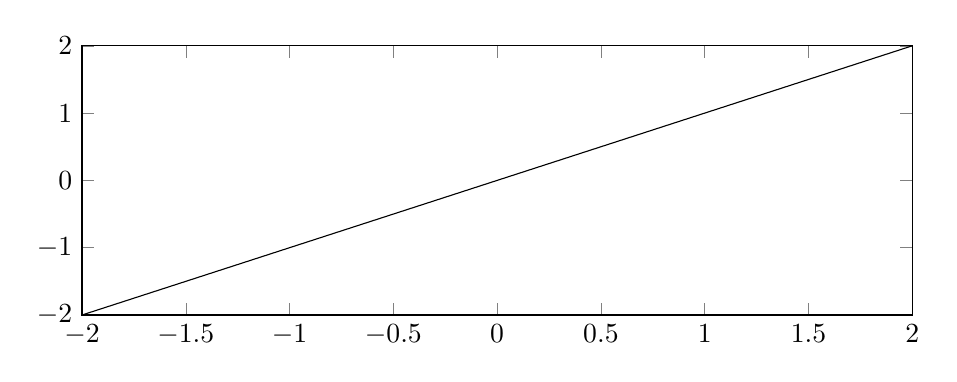
\begin{tikzpicture}
        \begin{axis}[
          width=\textwidth,
          height=5cm,
          xmin=-2,
          xmax=2,
          ymin=-2,
          ymax=2
        ]
          \addplot[black, domain=-2:2, samples=100] {x};
        \end{axis}
      \end{tikzpicture}
      \caption{Linear}
      \label{fig:plot1}
    \end{subfigure}
    \hfill
    \begin{subfigure}{0.3\textwidth}
        \centering
        \begin{tikzpicture}
          \begin{axis}[
            width=\textwidth,
            height=5cm,
            xmin=-2,
            xmax=2,
            ymin=-1.1,
            ymax=1.1,
            samples=100,
            xtick={-2,-1,0,1,2},
            ytick={-1,0,1},
            clip=false
          ]
            % Plot the sign function
            \addplot[black, thick, mark=none, domain=-2:0] {-1};
            \addplot[black, thick, mark=none, domain=0:2] {1};
            \draw (axis cs:0,-1) -- (axis cs:0,1);
          \end{axis}
        \end{tikzpicture}
        \caption{Sign Function}
        \label{fig:plot2}
      \end{subfigure}
    \hfill
    \begin{subfigure}{0.3\textwidth}
      \centering
      \begin{tikzpicture}
        \begin{axis}[
          width=\textwidth,
          height=5cm,
          xmin=-15,
          xmax=15,
          ymin=-1,
          ymax=1.1
        ]
          % Plot 3 data and settings
          \addplot[black, domain=-15:15, samples=100] {1/(1 + exp(-x))};
        \end{axis}
      \end{tikzpicture}
      \caption{Sigmoid}
      \label{fig:plot3}
    \end{subfigure}
  
    \medskip
  
    \begin{subfigure}{0.3\textwidth}
      \centering
      \begin{tikzpicture}
        \begin{axis}[
          width=\textwidth,
          height=5cm,
          xmin=-6.5,
          xmax=6.5,
          ymin=-1.1,
          ymax=1.1
        ]
          % Plot 4 data and settings
          \addplot[black, domain=-6.5:6.5, samples=100] {(exp(2*x)-1)/(exp(2*x)+1)};
        \end{axis}
      \end{tikzpicture}
      \caption{Tanh}
      \label{fig:plot4}
    \end{subfigure}
    \hfill
    \begin{subfigure}{0.3\textwidth}
      \centering
      \begin{tikzpicture}
        \begin{axis}[
            width=\textwidth,
            height=5cm,
            xmin=-2,
            xmax=2,
            ymin=-1.1,
            ymax=1.1
        ]
          % Plot 5 data and settings
          \addplot[black, domain=-2:2, samples=100] {max(x,0)};
        \end{axis}
      \end{tikzpicture}
      \caption{ReLU}
      \label{fig:plot5}
    \end{subfigure}
    \hfill
    \begin{subfigure}{0.3\textwidth}
      \centering
      \begin{tikzpicture}
        \begin{axis}[
            width=\textwidth,
            height=5cm,
            xmin=-2,
            xmax=2,
            ymin=-1.1,
            ymax=1.1
        ]
          % Plot 6 data and settings
          \addplot[black, domain=-2:2, samples=100] {max(min(x,1),-1)};
        \end{axis}
      \end{tikzpicture}
      \caption{Hard Tanh}
      \label{fig:plot6}
    \end{subfigure}
  
    \caption{Aktivierungsfunktionen}
    \label{fig:grid}
  \end{figure}
  
  TEXT FOLGT... 


\newpage
\subsubsection{Schichtenmodell}\label{subsec:neuronen:schichtenmodell}
  %\input{}
  TEXT FOLGT... 

\subsubsection{Loss-Function}

\newpage 
\subsection{Wie sind Neuronen miteinander verknüpft}\label{subsec:neuronen:verknuepfung_neuronen}  
%\input{}
Hier sollen die Weights erklärt werden

\subsubsection{Weights}\label{Weights}
  %\input{}
  TEXT FOLGT... 

\subsection{Fehler / Backpropagation Einführung}\label{subsec:neuronen:fehler_backpropagation}
Nur eine sehr knappe Einführung, da eigenes Kapitel für dieses Thema reserviert

